\chapter{SpaceRL: Our Knowledge graph reasoning proposal.}\label{chap:SpaceRL}

\chapterQuote{\hfill\textit{``Coffee, the finest organic suspension ever devised.''}}{--- Star Trek: Voyager}

\chapterAbstract{S}{oomething something, cool RL words.}
% hen a set of candidate triples has been obtained, the next step in Knowledge Graph completion is to classify every triple in said set to determine if it represents correct knowledge or not and, if found to be correct, added back to the KG in order to enrich it. In this chapter we introduce CAFE, our proposal for candidate triple classification. This chapter is structured as follows: Section~\ref{sec:cafe-intro} introduces it, Section~\ref{sec:cafe-proposal} presents the neighborhood-aware features that CAFE uses to discern between correct and incorrect triples, as well as the process it follows to do so, Section~\ref{sec:cafe-architecture} discusses its internal architecture and the design choices behind it, Section~\ref{sec:cafe-evaluation} shows the experiments that we carried out to assess the effectivity of CAFE, as well as their results; Section~\ref{sec:cafe-limitations} discusses its practical limitations; finally, Section~\ref{sec:cafe-summary} summarizes the chapter.

\section{Introduction}\label{sec:cafe-intro}
% This chapter presents CAFE~\cite{borrego2021}, our proposal for triple classification. CAFE covers the second main step in Knowledge Graph completion: once an adequately small set of candidate triples has been obtained, every triple in it must be carefully evaluated to determine whether or not it represents correct knowledge and, if so, added to the KG to enrich and expand it.

% CAFE works by transforming any possible triple into a numerical vector by using a novel set of neighborhood-aware features, which measure the correctness of a triple leveraging its context in a Knowledge Graph. By transforming all triples into vectors in this manner, CAFE trains and uses a binary classifier to discern between correct and incorrect triples.

% We thoroughly evaluate CAFE using several well-known Knowledge Graphs, and our evaluation shows that it is able to achieve a high precision in challenging, real-world scenarios, thus allowing for a trustworthy KG completion process.

% Over the course of this chapter, we continue to follow the running example introduced in Section~\ref{sec:theo-intro}.


\section{Our proposal}\label{sec:cafe-proposal}
% As previously described, the second major step when completing a Knowledge Graph consists of analyzing the set of possible candidate triples, assessing which ones represent correct knowledge, and adding them back to the KG in order to augment it. In this step, it is important to achieve a high precision, in order to have a Knowledge Graph completion process that is as trustworthy as possible~\cite{shen2022overview}.

% To carry out this process, we have devised CAFE, a technique that classifies candidate triples into correct or incorrect ones. Given a Knowledge Graph and a set of candidate triples, CAFE evaluates each one of them and assigns them a binary label, denoting whether it should be considered correct and added to the Knowledge Graph, or incorrect and discarded. CAFE does this by defining a set of neighborhood-aware features, which checks for shared neighborhoods at several distance levels and under certain conditions, under the assumption that the entities in correct triples usually have a higher degree of overlap in their neighborhoods. Then, using these features, each candidate triple is converted into a numerical vector. Finally, CAFE trains a number of neural classification models using these vectors to learn to separate correct triples from incorrect ones. In the following subsections, we describe the features and architecture of CAFE in detail.

\subsection{Neighborhood-aware features}\label{sec:cafe-features}
% We propose a set of neighborhood-aware features that takes neighborhood subgraphs, reachable entities and paths into account. Due to the large number of possible variations of each feature, we present our feature set in terms of groups of features. Each group can be parameterized to obtain a specific feature, which we call an instance of the feature group.

% For the sake of example, we illustrate a possible instance of every feature group and its value using the example triple $example = $\tripleSty{(Daniel Radcliffe, plays, Harry Potter)}, and the KG shown in Figure~\ref{fig:kg-potter}.

% \featgroup{Number of entities in the neighborhood subgraph of size \texorpdfstring{$n$}{n} of the source entity in the triple.}
% {n}
% {|\Eset{}_s^n|}
% {fig:kg-potter}
% {2}
% {$|\{$\textit{Daniel Radcliffe, Harry Potter and the Goblet of Fire (movie), Harry Potter and the Prisoner of Azkaban (movie), Harry Potter and the Goblet of Fire (book), Harry Potter and the Prisoner of Azkaban (book)}$\}| = 5$}


% \featgroup{Number of entities in the neighborhood subgraph of size \texorpdfstring{$n$}{n} of the target entity in the triple.}
% {n}
% {|\Eset{}_t^n|}
% {fig:context-examples-b}
% {3}
% {$|\{$\textit{Harry Potter, J.K. Rowling, Harry Potter and the Goblet of Fire (book), Harry Potter and the Prisoner of Azkaban (book), Robin Ellacott, Hermione Granger}$\}| = 6$}

% \featgroup{Degree of N-path centrality of the source entity in the triple.}
% {n}
% {\frac{|\Eset{}_s^n|}{|\Eset| - 1}}
% {fig:context-examples-a}
% {1}
% {$|\{$\textit{Harry Potter and the Goblet of Fire (movie), Harry Potter and the Prisoner of Azkaban (movie)}$\}| / (13 - 1) = 2 / 12 \approx 0.17$}

% \featgroup{Degree of N-path centrality of the target entity in the triple.}
% {n}
% {\frac{|\Eset{}_t^n|}{|\Eset| - 1}}
% {fig:context-examples-b}
% {1}
% {$|\{$\textit{Harry Potter and the Goblet of Fire (book), Harry Potter and the Prisoner of Azkaban (book)}$\}| / (13 - 1) = 2 / 12 \approx 0.17$}

% \featgroup{Number of common entities between the neighborhood subgraph of size \texorpdfstring{$n$}{n} of the source entity and the neighborhood subgraph of size \texorpdfstring{$m$}{m} of the target entity in the triple.}
% {n, m}
% {|\Eset{}_s^n \cap \Eset{}_t^m|}
% {fig:context-examples}
% {2, 3}
% {$|\{$\textit{Harry Potter and the Goblet of Fire (book)}, \textit{Harry Potter and the Prisoner of Azkaban (book)}$\}| = 2$}

% \featgroup{Jaccard index of similarity between the entities in the neighborhood subgraph of size \texorpdfstring{$n$}{n} of the source entity and the neighborhood subgraph of size \texorpdfstring{$m$}{m} of the target entity in the triple.}
% {n, m}
% {jaccard(\Eset{}_s^n, \Eset{}_t^m)}
% {fig:context-examples}
% {2, 3}
% {$|\{$\textit{Harry Potter and the Goblet of Fire (book), Harry Potter and the Prisoner of Azkaban (book)}$\}|$~$/$~$|\{$\textit{Daniel Radcliffe, Harry Potter and the Goblet of Fire (movie), Harry Potter and the Prisoner of Azkaban (movie), Harry Potter and the Goblet of Fire (book), Harry Potter and the Prisoner of Azkaban (book), Harry Potter, J.K. Rowling, Robin Ellacott, Hermione Granger}$\}| = 2~/~9 = 0.22$}

% \featgroup{Adamic-Adar index of closeness between the neighborhood subgraphs of size \texorpdfstring{$n$}{n} of the source and target entities in the triple.}
% {n}
% {\sum_{e \in \nearby{s}{n} \cap \nearby{t}{n}}{\frac{1}{log |\nearby{e}{n}|}}}
% {fig:context-examples}
% {2}
% {$\frac{1}{log |\nearby{\textit{\footnotesize Harry Potter and the Goblet of Fire (book)}}{2}|} = \frac{1}{log |3|} \approx 2.09$}

% \featgroup{Number of reachable entities through the relation \texorpdfstring{$r$}{r} at distance \texorpdfstring{$n$}{n} from the source entity in the triple.}
% {r, n}
% {|Reachable(s, r, n)|}
% {fig:context-examples-a}
% {\textit{hasPrequel}, 2}
% {$|\{$\textit{Daniel Radcliffe, Harry Potter and the Prisoner of Azkaban (movie)}$\}| = 2$}

% \featgroup{Number of reachable entities through the relation \texorpdfstring{$r$}{r} at distance \texorpdfstring{$n$}{n} from the target entity in the triple.}
% {r, n}
% {|Reachable(t, r, n)|}
% {fig:context-examples-b}
% {\textit{created}, 2}
% {$|\{$\textit{Harry Potter,Hermione Granger, Robin Ellacott}$\}| = 3$}

% \featgroup{Number of common reachable entities through the relation \texorpdfstring{$r$}{r} from the source entity at distance \texorpdfstring{$n$}{n} and from the target entity at distance \texorpdfstring{$m$}{m}.}
% {r, n, m}
% {\\|Reachable(s, r, n) \cap Reachable(t, r, m)|}
% {fig:context-examples}
% {\textit{created}, 2, 3}
% {$|\{$\textit{Daniel Radcliffe}$\} \cap \{$\textit{Harry Potter, Hermione Granger, Robin Ellacott}$\}| = 0$}

% \featgroup{Jaccard index of similarity between the reachable entities through the relation \texorpdfstring{$r$}{r} from the source entity at distance \texorpdfstring{$n$}{n}, and those reachable through the relation \texorpdfstring{$r$}{r} from the target entity at distance \texorpdfstring{$m$}{m}.}
% {r, n, m}
% {\\jaccard(Reachable(s, r, n), Reachable(t, r, m))}
% {fig:context-examples}
% {\textit{created}, 2, 3}
% {$|\emptyset|$~$/$~$|\{$\textit{Harry Potter, Hermione Granger, Robin Ellacott}$\}| = 0~/~3 = 0$}


% \featgroup{Number of distinct paths of length \texorpdfstring{$n$}~ between the source and the target entity in the triple, using  relations \texorpdfstring{$r_1, \ldots, r_n$}{r1, ..., rn}.}
% {n, r\textsubscript{1}, \ldots, r\textsubscript{n}}
% {|\kgpathP{s}{t}{r_1,\ldots, r_n}|}
% {fig:kg-example}
% {4, \textit{starred\_in, based\_on, writer, created}}
% {$1$, as there is one path of length 4 between the entities \textit{Daniel Radcliffe} and \textit{Harry Potter} that matches the given relations}

% % Discussion of features
% The rationale behind this set of features is manifold. Regarding $f_1$ and $f_2$, knowing the size of the neighborhood of an entity can be helpful to determine whether said neighborhood encompasses relevant information. For instance, our hypothesis is that very large neighborhoods tend to contain a higher amount of unrelated information. The same idea is leveraged in $f_3$ and $f_4$, which provide normalized indices of centrality with respect to the total amount of entities in the KG. Following the previous reasoning, we hypothesize that entities with large indices of centrality (i.e. highly connected to other entities) will yield less useful information. Meanwhile, feature groups $f_5$, $f_6$ and $f_7$ measure the degree of overlap that exists in the neighborhoods of the two entities, both in absolute and in relative terms, under the assumption that correct triples have a higher degree of overlap between the neighborhoods of their entities.

% The previously discussed feature groups do not consider the specific relations involved. However, we deem it reasonable to assume that some relations may be more useful than others to determine whether a triple is correct, depending on their specific semantics. For example, having one or more children in common can be an indication of a marriage, while having the same nationality is not. In order to exploit this fine-grained information, feature groups $f_8$, $f_9$, $f_{10}$ and $f_{11}$ are similar to the previously discussed groups but restrict themselves to only one relation. These groups are computed for every relation in a KG.

% Finally, feature group $f_{12}$ allows CAFE to find the number of paths that exist between two entities for any given relations. It is our intuition that correct triples have more alternative paths between the two entities they contain than false ones.

\subsection{Workflow}
% Our proposal, CAFE, receives a KG and a set of relations from that KG as input, and outputs a classification model for each of the provided relations. These models are able to determine if a given triple that represents an instance of the relation is correct and should belong to the KG. Its workflow is depicted in Figure~\ref{fig:workflow-cafe} and, in the following, we describe each of its steps.

% \begin{figure}[htp]
%     \centering
%     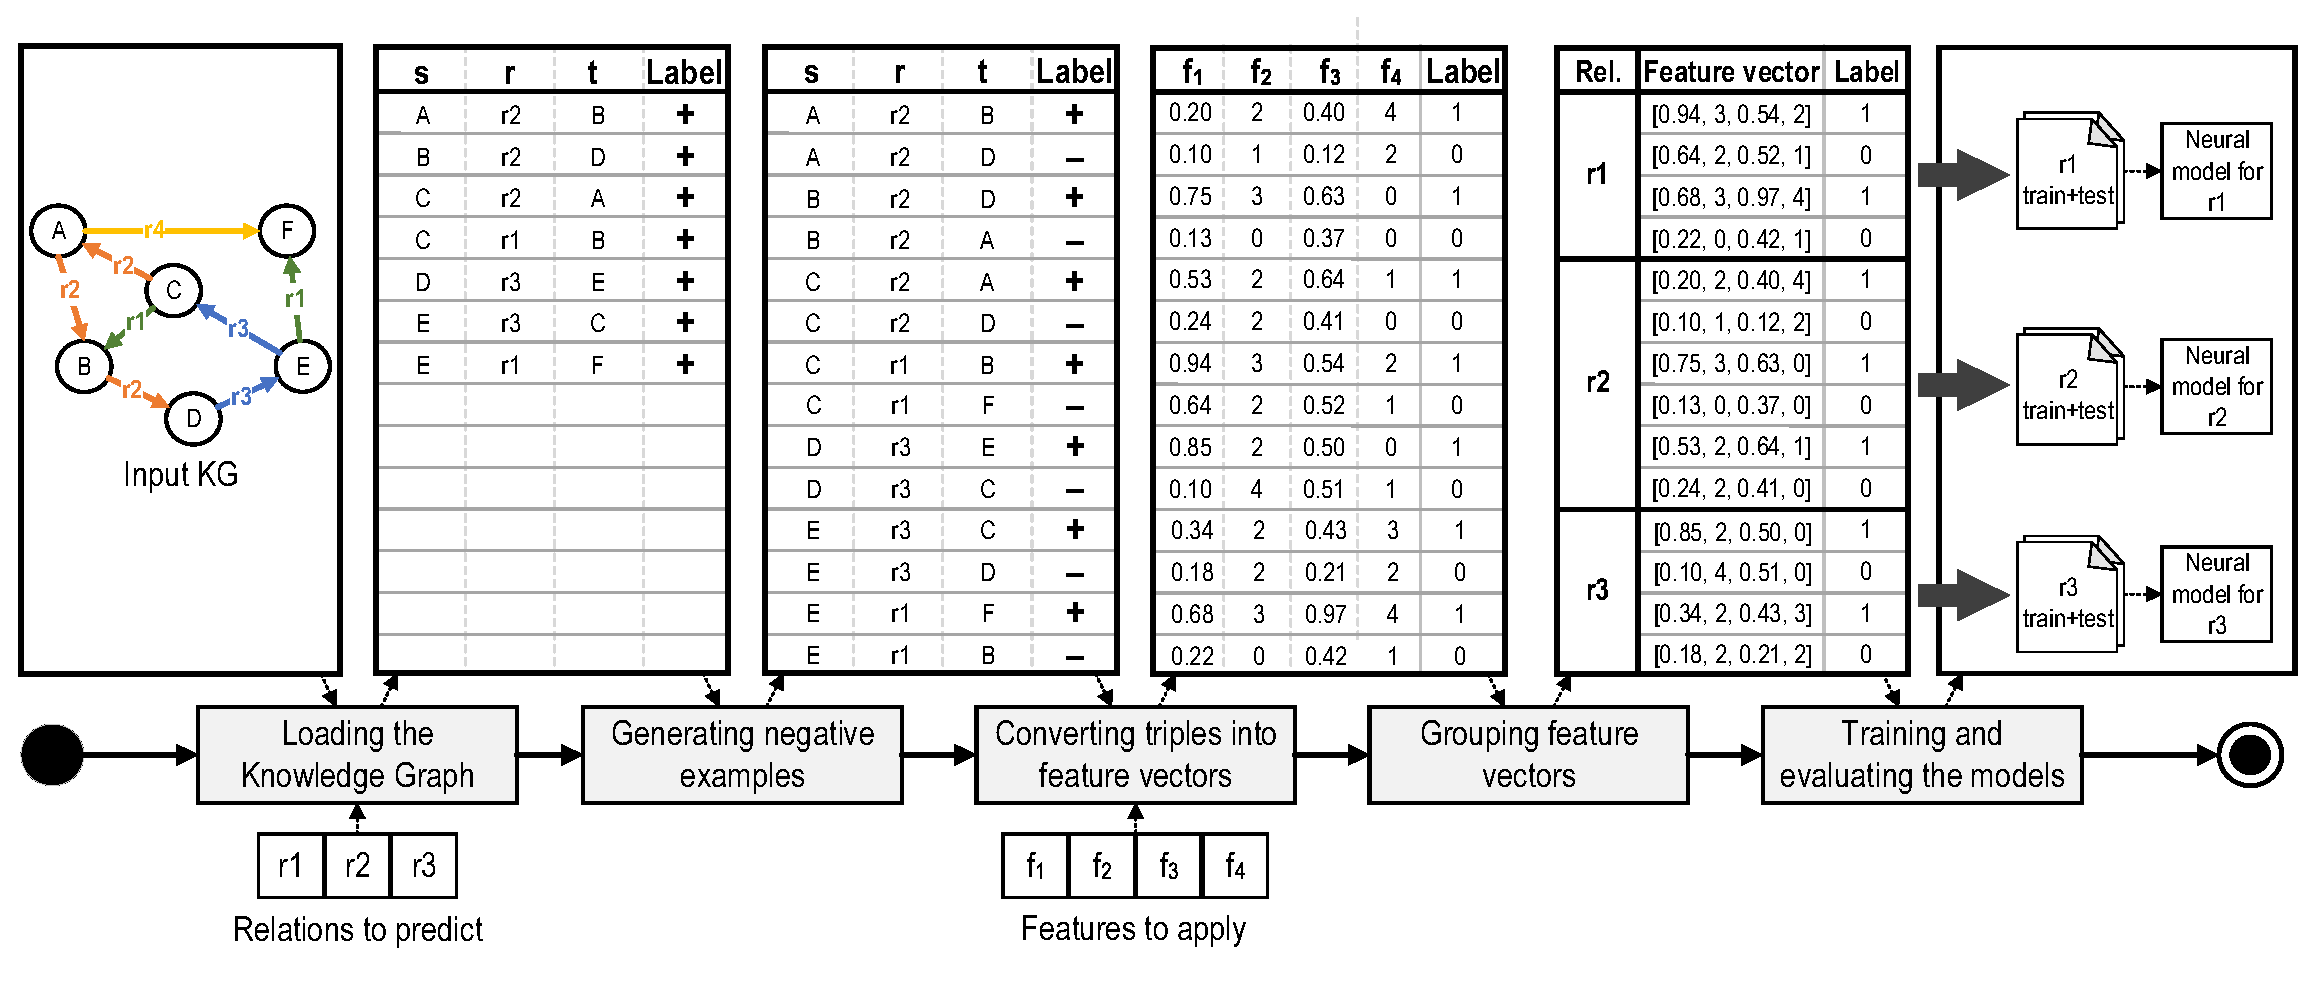
\includegraphics[width=\textwidth]{fig/cafe/workflow}
%     \caption{In-depth view of the CAFE workflow}
%     \label{fig:workflow-cafe}
% \end{figure}

% \begin{itemize}
%     \item \textbf{Loading the Knowledge Graph:} CAFE internally stores the input KG in the form of \triple{} triples, using an efficient data structure based on hash tables, which is suitable for a high frequency of read operations due to its O(1) lookup times. The triples that contain relations for which a predictive model does not need to be generated are still taken into account when computing features, since they may provide valuable predictive information, but they are not transformed into feature vectors in the following steps.\\
    
%     \item \textbf{Generating negative examples:} A Knowledge Graph contains only positive information, i.e., it contains examples of the occurrence of a relation $r$ between two entities. However, it does not contain explicit information about pairs of entities for which $r$ does not hold. Our proposal relies on a classification model that requires negative examples for training, which means that a number of negatives for each positive triple must be produced. To accomplish this, we follow the type-constrained local closed world assumption \cite{bansal2020negatives}, i.e., we generate negative examples from every triple \triple{} present in a KG by replacing their target entity $t$ with a different one, $t'$, such that the resulting triple \negtriple{} does not exist in the KG. Furthermore, to preserve the range of each relation, we randomly choose $t'$ such that there exists some other triple in the KG where $t'$ appears as the target entity for the relation $r$. This is known as type constraint.\\

%     In the example depicted in Figure \ref{fig:kg-potter}, a valid negative example is \tripleSty{(Hermione Granger, appears\_in, The Cuckoo's Calling)}, since we know that \tripleSty{The Cuckoo's Calling} is a valid target for the relation \tripleSty{appears\_in}. However, \tripleSty{(Hermione Granger, appears\_in, Daniel Radcliffe)} would not be allowed as a negative example, because \tripleSty{Daniel Radcliffe} never appears as the target of the relation $appears\_in$.\\
    
%     It can be argued that generating negative evidence in this manner can produce false negatives by mere chance, i.e., statements that are deemed incorrect but that are true in the real world. While this is indeed plausible, it is generally accepted~\cite{ji2015, lin2015, socher2013} that the chances of this happening are very low and, as a consequence, the possible effects on the final results are not significant.\\

%     \item \textbf{Converting triples into feature vectors:} Once negative examples have been generated, our feature set is instantiated and applied to all triples. For all feature groups, we obtain all possible feature instances by applying all possible combinations of the values of their parameters. Each feature instance assigns a real number to each triple. Therefore, applying several features to a triple results in a feature vector. Each position of the feature vector represents that real number that the corresponding feature assigned to the triple.\\

%     It is important to note that, to compute features on a positive training triple, we temporarily remove it from the KG, since not doing so would result in trivial prediction models such as ``a person plays a character if there exists a triple in the KG stating that the person plays that character''.\\\newpage

%     \item \textbf{Grouping feature vectors:} The previous step computes feature vectors of triples. Since these triples can be either positive or negative, the feature vectors are accordingly labeled as positive or negative. Based on the labeled feature vectors, we train a classification model for each relation that predicts whether a triple should be added to the KG. We do this in order to allow the models to capture meaningful and distinctive information for every relation: even though the same set of features is applied to all triples, some features might have more predictive power for a relation, and other features may be more helpful for a different one.\\
    
%     \item \textbf{Training and evaluating the models:} For every relation that we predict, we create one or more neural models, where each model focuses only on the features that are obtained from a certain neighborhood size. Thus, using only neighborhood subgraphs of size 1 results in one model, using neighborhood subgraphs of size of up to 2 results in two models, and so on. This allows each model to capture the specific information that every neighborhood size may yield. To combine two or more models, we use an additional combination layer to produce a single output.

%     The neural models are trained using the labeled feature vectors in the training split for the desired relation, where each model receives only the features corresponding to its assigned neighborhood size, and the label or ground truth is shared among them. Prior to training our models, we first remove any individual features that have the exact same value in every feature vector and thus lack any predictive power. An example of this are path-based features ($f_{12}$), since only a small subset of all possible paths of fixed length occur between two given entities, and as a consequence most of them have a value of 0.
    
%     It is important to note that we use neural classification models because they have been shown to consistently achieve satisfactory results in many different classification tasks~\cite{aggarwal2012, yadav2019, ayala2020}, although other classification models that make use of our features could be used in this step.
% \end{itemize}

\section{Software Architecture}\label{sec:cafe-architecture}
% We show the internal class architecture of CAFE in Figure~\ref{fig:cafe-diagram}, and its data workflow is displayed in Figure~\ref{fig:cafe-flow}. We further describe and discuss the architecture of CAFE in the following.

% \begin{figure}[!htp]
%     \centering
%     \includesvg[width=1.0\textwidth]{fig/cafe/CAFE-classes}
%     \caption{Architecture of CAFE}
%     \label{fig:cafe-diagram}
% \end{figure}

% \begin{figure}[!htp]
%     \centering
%     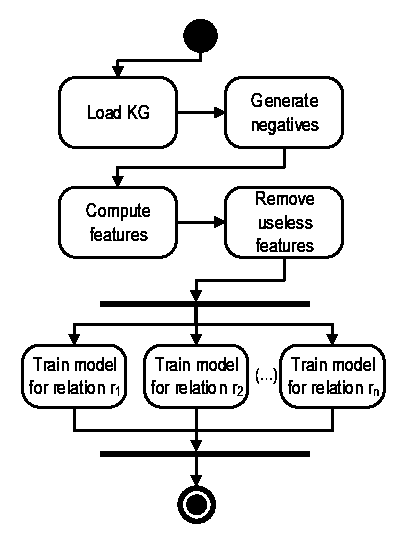
\includegraphics[width=.45\textwidth]{fig/cafe/CAFE-flow}
%     \caption{Workflow of CAFE}
%     \label{fig:cafe-flow}
% \end{figure}

% The main flow of CAFE is coordinated by the class \textit{ParallelWorker}. This class can be configured to use a certain number of threads, and then internally spawns processes to parallelize the different tasks done by CAFE. This is done by splitting the total number of triples in the KG between the different threads, since the processing of triples can be done concurrently for the most part, as shown in Figure~\ref{fig:cafe-flow}. 

% The method \textit{genNegs} produces negative triples using the \textit{NegativeGenerator} class and a generation strategy, since they are necessary to train the classification models.

% Then, the method \textit{compFeats} transforms every triple in the KG into a labeled feature vector, using a series of neighborhood-aware features that leverage the similarities of the neighborhoods of two entities in a KG. This is done by measuring the similarities of the entity neighborhoods of the source and target of a triple, using measures such as the Jaccard index of similarity, analyzing the size of such neighborhoods using measures such as the Adamic-Adar index; as well as assessing the overall connectivity of the entities of a triple using the N-path centrality index.

% The method \textit{filtFeats} removes the features that have the same value in all labeled vectors, since they have no predictive power. Finally, method \textit{getClassifier} trains and returns a neural classifier for a given set of labeled vectors, corresponding to a certain relation in the KG. Given that the work done by these methods is usually carried out in an independent manner for each triple, it is parallelized among different execution threads.

% Class \textit{ParallelWorker} uses other classes by means of composition to perform specialized tasks: Class \textit{NegativeGenerator} provides a unified interface to easily generate a negative triple in a KG following one of the available strategies, which are implemented using \textit{NegGenerationStrategy} classes.

% Class \textit{KGLoader}, through its \textit{load} method, is used to read and write KGs in different formats, namely: N3, Turtle, and RDF/XML.

% Class \textit{FeatureVectorCalculator} is responsible for applying the previously discussed catalogue of features to any given triple using the method \textit{getVec}, resulting in a labeled vector for that triple. The catalogue of available features can be easily expanded thanks to the \textit{Feature} class, since each individual feature is implemented as an instance of that class.

% Class \textit{FeatureFilterer} specializes in removing useless features from a feature vector, i.e., those that share the same value in all vectors and thus have no predictive power. Method \textit{filtFeat} receives the labeled vector to be processed and a set of all other labeled vectors, to allow for the multithreaded processing of different labeled vectors simultaneously.

% Finally, the \textit{NeuralClassifier} class produces, trains and evaluates the neural models that determine whether a triple is correct. These models receive as input the feature vector generated from the triple in question, and outputs a confidence value between 0 and 1. The models used by CAFE have three feed-forward layers with 1024, 512 and 256 neurons each. The method \textit{initialize} produces a new model for a certain relation, to allow it to specialize in the specific details of said relation, which may be different to other relations present in the KG. The method \textit{train} receives the training set of labeled vectors resulting from processing a KG with the \textit{ParallelWorker}, and uses them to train the classification model. This method uses a learning rate of 0.001, a dropout of 0.1 for all layers, a batch size of 16 and 100 epochs, as these parameters have been proven to yield satisfactory results in some of our previous work \cite{borrego2021}. Then, all vectors in the testing set are evaluated using the \textit{predict} method.

% Throughout the whole process, the \textit{Settings} class is queried to retrieve the configuration parameters set by the user, e.g., the relative sizes of the training and testing splits, or the negative generation strategy to use.

% CAFE has two main dependencies with external libraries: NetworkX \cite{hagberg2008networkx}, which is used to internally store the KG and apply graph-based algorithms to compute the different features; and TensorFlow \cite{tensorflow2015}, which is used to create, train and apply the neural classification models.

\subsection{Design and performance considerations}
% The architecture of CAFE shares some common patterns and design decisions with that of CHAI, described in the previous chapter. Most classes only need to be instantiated once throughout the execution of CAFE and, for this reason, we have decided to turn them into singletons for simplicity of use and to minimize the use of memory.

% There are, nonetheless, a number of classes that clearly must allow multiple instances of them to exist, in order to represent variations of the same concept. A prime example of this is the Feature class: all features share the same interface, since they receive a triple and the KG that contains it and produces a numeric value. However, in order to accommodate all features defined in Section~\ref{sec:cafe-features}, each one of them exists as an instance of Feature.

% Another example is the possible existence of multiple negative generation strategies, where one must be chosen at runtime according to the selection of the user. In both cases, they are accessed through auxiliary classes that act as catalogues, automatically detecting and loading all instances of the catalogued classes. 

% Given that CAFE is a very computationally intensive system, several optimizations have been made to make the best possible use of the resources of the system it runs on. Due to the fact that computing a feature vector for a triple can be done independently of all other triples in a KG, this task is parallelized and evenly distributed among all available cores in a CPU. This, however, comes at the cost of ensuring that all singletons in the system are thread-safe, given that they will be accessed by multiple processes at the same time.

% Finally, it is important to note that all features defined by CAFE are deterministic, and will always return the same value for the same triple in a KG. Most features only analyze one of the entities in a triple at a time, and thus are re-computed very often for the same entity. For this reason, we have implemented a thread-shared caching strategy, in which the result of applying a feature to a triple is stored into a cache that is accessed by all threads. This allows CAFE to significantly reduce the number of calculations that must be performed when processing a KG.

\section{Evaluation}\label{sec:cafe-evaluation}
% In this section, we present the evaluation that we carried out to assess the performance and effectiveness of CAFE. First, we introduce the Knowledge Graphs on which CAFE was applied and an overview of their main characteristics. Next, we explain the methodology that we used to evaluate CAFE. Finally, we show and discuss the results of our evaluation.

\subsection{Experimental data}
% We evaluated our proposal using four KGs provided by the freely available AYNEC-DataGen~\cite{ayala2019} tool: FB13-A, WN11-AR, WN18-AR and NELL-AR. These KGs are based on the well-known FB13, WN11 \cite{socher2013}, WN18~\cite{bordes2014}, and a subset of NELL proposed in \cite{gardner2015}. However, they have been processed to remove reciprocal relations detected by AYNEC, i.e., relations $r$ and $r'$ such that, if $(s, r, t)$ exists, then $(t, r', s)$ also exists very frequently. Additionally, relations that amount to less than 5\% of the total number of triples in the graph have been removed.

% These evaluation KGs originally contained one negative example per each positive triple in both their training and testing splits. In order to study how the KG completion techniques perform when presented with a much higher volume of negative evidence, we created versions of these graphs whose testing splits contained 10 negative examples per positive, using the AYNEC-DataGen tool. We believe that this is a more realistic scenario, since a much higher number of negative examples per positive triple is typically expected in real-world KG completion tasks~\cite{borrego2019}. To avoid confusion, we denote these versions as FB13-A-10, WN11-AR-10, WN18-AR-10 and NELL-AR-10.

% For FB13-A-10, WN11-AR-10 and WN18-AR-10, we aimed to predict all possible relations, and for NELL-AR-10 we focused on the same subset of 10 relations that were used to evaluate SFE~\cite{gardner2015}. However, in the latter KG, one relation was removed by AYNEC for being the reciprocal of another relation, leaving 9 relations for evaluation. In the specific case of FB13-A-10, we transferred 25\% of the training triples over to the testing set in order to provide testing examples for some relations, as they were not available in the original KG as introduced in \cite{socher2013}. Table \ref{table:cafe-datasets} provides an overview of the aforementioned KGs. In the case of NELL-AR-10, we show in parentheses the amount of triples and relations that were considered for evaluation, although the entire graph was used for computing features.

% \begin{table}
    % \footnotesize
    \begin{center}
    \begin{tabular}{ >{\raggedright\arraybackslash}M{3.5cm} | M{2.5cm} | M{2.5cm} | M{1.75cm} | M{1.75cm} }
    \centering \textbf{KG} & \textbf{Training triples} & \textbf{Test triples} & \textbf{Entities} & \textbf{Relations} \\
    % actualizado marzo 2021
    \hline
    FB13-A-10 & 228,172 & 481,457 & 74,998 & 13 \\ 
    \hline
    WN11-AR-10 & 77,948 & 198,231 & 38,195 & 9 \\
    \hline 
    WN18-AR-10 & 71,984 & 183,051 & 40,943 & 11 \\
    \hline 
    NELL-AR-10 & 86,971 (1,451) & 219,374 (5,083) & 53,934 & 148 (9) \\
    \end{tabular}
    \caption{Overview of the KGs used for evaluating CAFE}
    \label{table:cafe-datasets}
    \end{center}
\end{table}

\subsection{Experimental setup}
% A neural prediction model was created for every relation of interest and trained using its corresponding training set. Then, the model was applied to all feature vectors in the test set, and we compared the expected label (which denotes whether it represents a correct triple or not) against the label that was produced by our model. We report our results in terms of precision, recall and F1, in order to determine how effective our proposal is when determining the correctness of a given triple.

% We evaluated three versions of CAFE, denoted CAFE$_1$ to CAFE$_3$, which were limited to using feature instances that exploited neighborhood subgraphs and paths of a maximum size of 1, 2, and 3, respectively. This was done in order to study how using larger neighborhoods affects the effectiveness of CAFE.

% There exist many different KG completion proposals, and they often use different evaluation metrics \cite{speranskaya2020}. Due to this, it is very difficult to perform a comparison across a large number of them in a manner that is fair and rigorous. For this reason, we used TransE~\cite{bordes2013}, TransD~\cite{ji2015}, TransH~\cite{wang2014}, TransR~\cite{lin2015}, Analogy~\cite{liu2017}, SimplE~\cite{kazemi2018} and RotatE~\cite{sun2019} as baselines for our evaluation, since they are some of the most well-known state-of-the-art KG completion proposals. In order to provide a common evaluation environment for these different proposals, we used the OpenKE \cite{han2018} framework to train and evaluate these proposals using the previously discussed Knowledge Graphs. Additionally, since these proposals usually report metrics like MRR and Precision@N, we used the utilities provided by OpenKE to obtain binary labels for the testing triples, by setting a likelihood threshold in a way that optimized the classification results.

% We selected the following values for the hyperparameters of our neural models: 3 layers with 1024, 512 and 256 neurons each, learning rate of 0.001, batch size of 16, dropout of 0.1 for all layers, 100 epochs and validation ratio of 10\%. When two or more models were to be combined, we joined their results using a hidden layer with 3 neurons and an output layer with a single neuron. These values for the hyperparameters were chosen using a hold-out or ``dev'' set for the FB13-A-10 KG, and all KGs were then evaluated using the same hyperparameters. We chose them because they provided satisfactory results in our empirical tests.

% All our experiments were conducted on a computer equipped with an Intel Core i9-9900K CPU, 32GB of RAM and an Nvidia RTX 2080 Ti GPU.

\subsection{Results and discussion}
% In Figure \ref{fig:cafe-boxes}, we show the evaluation results for CAFE$_1$, CAFE$_2$, CAFE$_3$, and the related state-of-the-art proposals. For the sake of clarity, this Figure only displays the F1 values for each technique. Additionally, Table \ref{fig:cafe-table-results} shows the detailed results for all relations in every KG and for all metrics under evaluation.

% \begin{figure}[!htp]
%     \centering
%     \def\subfigscale{0.6\textwidth}
    
%     \subfigure[FB13-A-10]{
%         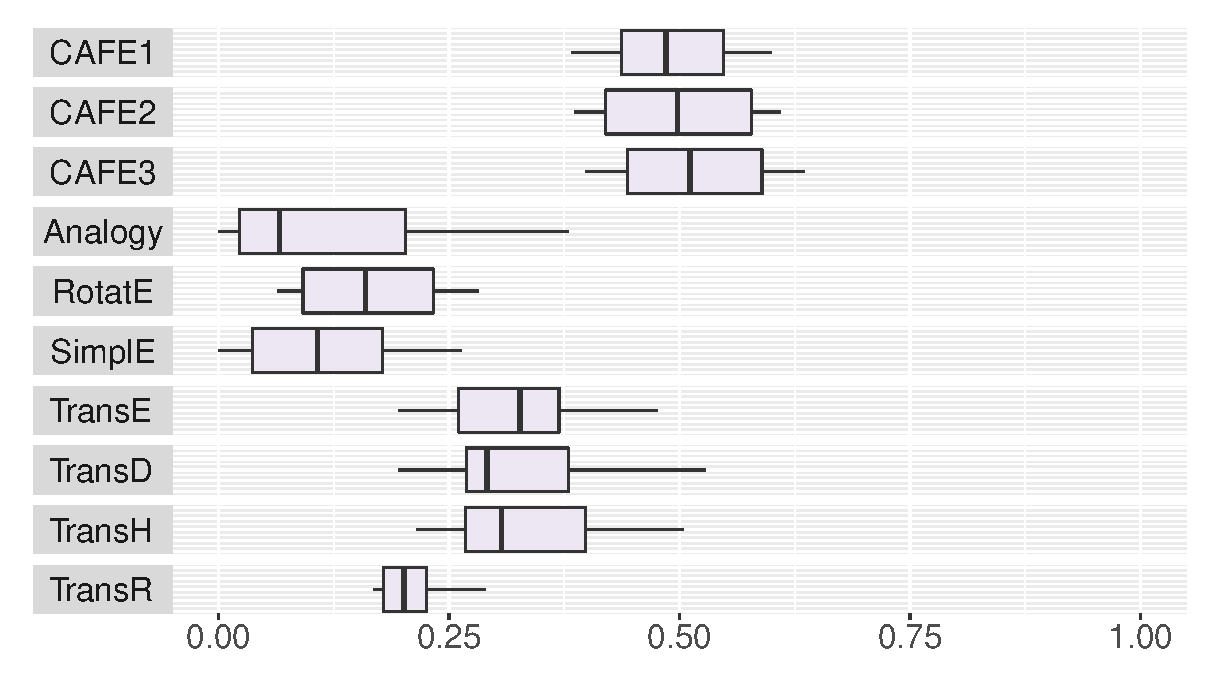
\includegraphics[width=\subfigscale]{fig/cafe/boxes/FB13-A-10}
%         \label{fig:box-FB13-A-10}
%     }\\
%     \subfigure[NELL-AR-10]{
%         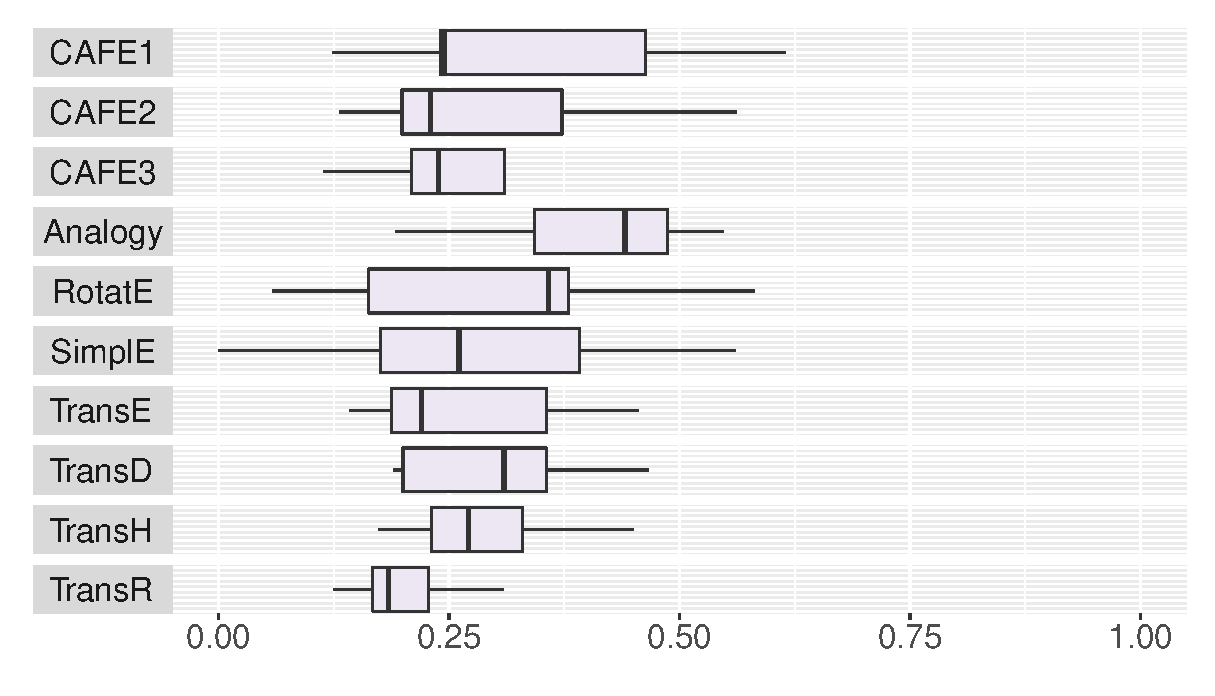
\includegraphics[width=\subfigscale]{fig/cafe/boxes/NELL-AR-10}
%         \label{fig:box-NELL-AR-10}
%     }\\
%     \subfigure[WN11-AR-10]{
%         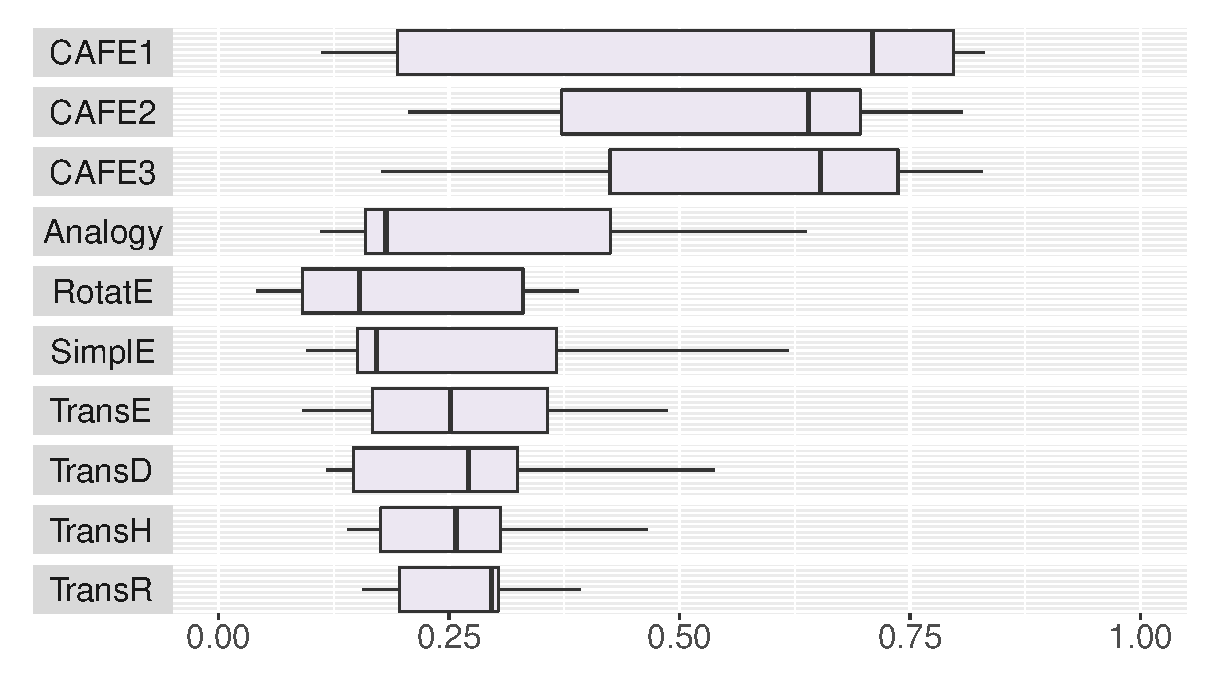
\includegraphics[width=\subfigscale]{fig/cafe/boxes/WN11-AR-10}
%         \label{fig:box-WN11-AR-10}
%     }

%     \caption{F1 comparison between CAFE and other proposals}
%     \label{fig:cafe-boxes}
% \end{figure}

% \begin{figure}[!htp]\ContinuedFloat
%     \centering
%     \def\subfigscale{0.6\textwidth}
    
%     \subfigure[WN18-AR-10]{
%         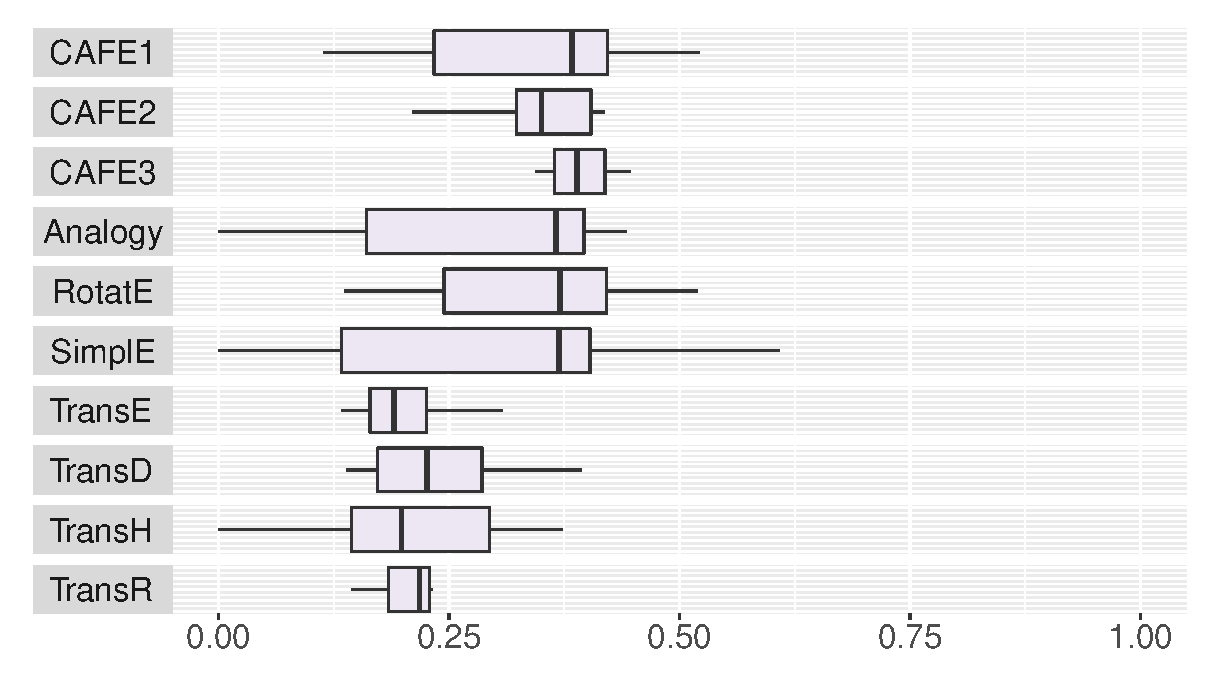
\includegraphics[width=\subfigscale]{fig/cafe/boxes/WN18-AR-10}
%         \label{fig:box-WN18-AR-10}
%     }\\
    
%     \caption{F1 comparison between CAFE and other proposals (cont.)}
% \end{figure}

% \begin{figure}[!htp]
%     \centering
%     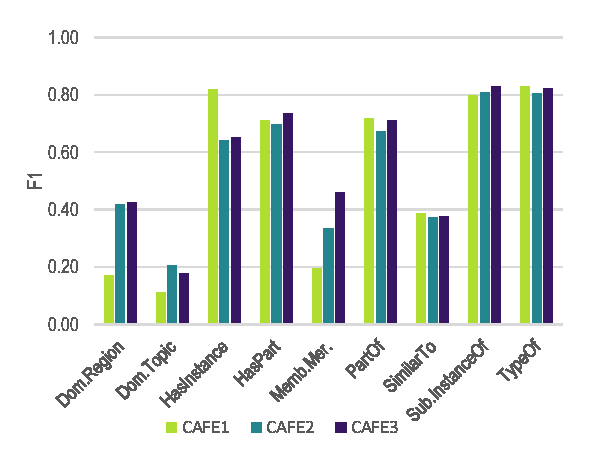
\includegraphics[width=.75\textwidth]{fig/cafe/wn11_bars}
%     \caption{F1 scores in the WN11-AR-10 KG}
%     \label{fig:cafe-wn11-bars}
% \end{figure}

% Our results show that CAFE is able to match the performance of state-of-the-art proposals, and in many cases achieve higher values on the metrics under evaluation. In the cases of FB13-A-10 (Figure \ref{fig:box-FB13-A-10}) and WN18-AR-10 (Figure \ref{fig:box-WN18-AR-10}), CAFE can reach or surpass the F1 scores achieved by other proposals in a consistent manner. CAFE also provides better results in the WN11-AR-10 (Figure \ref{fig:box-WN11-AR-10}) KG, although with a higher degree of variability, and matches the performance of the rest of the analyzed techniques in the NELL-AR-10 (Figure \ref{fig:box-NELL-AR-10}) KG. These results show that CAFE can be more effective than other proposals in challenging classification scenarios.

% \newpage
% \clearpage

% \begin{table}[H]
%     \centering
%     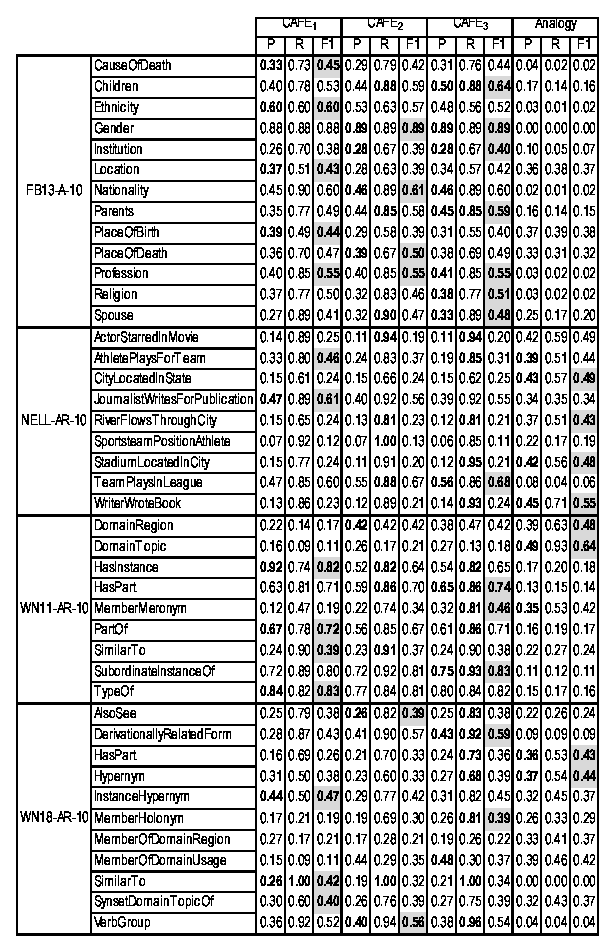
\includegraphics[height=0.8\paperheight,right]{fig/cafe/table-cafe-left}%
%     \caption{Detailed CAFE results}
%     \label{fig:cafe-table-results}
% \end{table}  
% \begin{table}[H]\ContinuedFloat
%     \centering
%     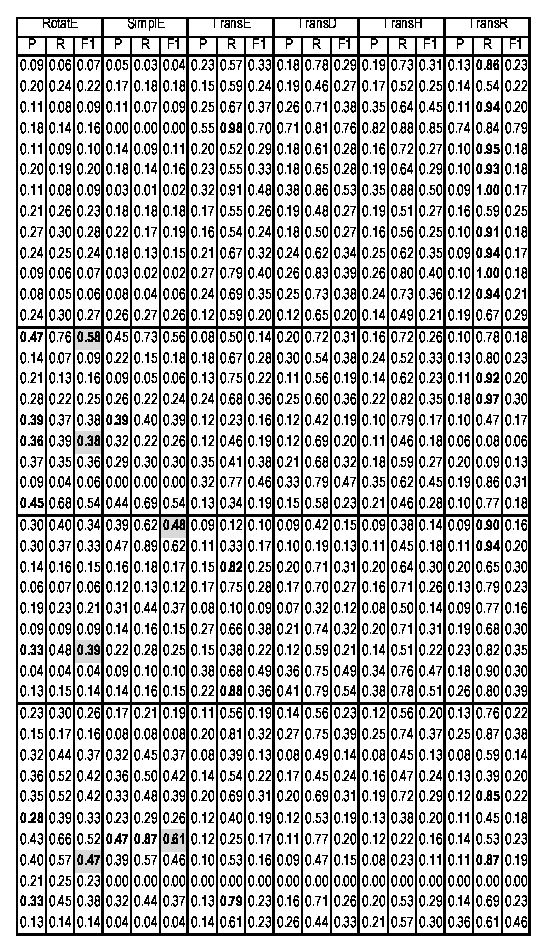
\includegraphics[height=0.8\paperheight,left]{fig/cafe/table-cafe-right}%
%     \caption{Detailed CAFE results (cont.)}
% \end{table}


% \newpage

% Table \ref{fig:cafe-table-results} displays that, in general, both a satisfactory precision and recall can be achieved, and thus we consider that CAFE is generally effective. However, there exists a number of relations for which a very high precision value is obtained at the expense of a lower recall or vice-versa, resulting in a typical precision-recall trade-off. We also observe that the nature of every individual relation has a significant impact in the results, since some of them are harder to predict than others. Such is the case of the relation \textit{cause\_of\_death}, since learning to predict the cause of the death of a person with a very high effectiveness would be a remarkable achievement that unfortunately falls out of the scope of this work. We further discuss this limitation in Section \ref{sec:cafe-limitations}.

% Regarding the question of how using different neighborhood sizes affects the effectiveness of CAFE, Figure~\ref{fig:cafe-boxes} shows that the metrics under evaluation are generally higher for CAFE$_2$ than for CAFE$_1$, but the same cannot always be said for CAFE$_3$ and CAFE$_2$. Indeed, metrics appear to remain stagnant or even decrease when using larger neighborhoods in some cases. For example, in FB13-A-10 (Figure \ref{fig:box-FB13-A-10}), we do not observe a significant increase in effectiveness when using larger neighborhood subgraphs, which suggests that the most useful information is readily available in the immediate vicinities of the relevant entities. In the cases of WN11-AR-10 (Figure \ref{fig:box-WN11-AR-10}) and WN18-AR-10 (Figure \ref{fig:box-WN18-AR-10}), an improvement is observed when using neighborhoods of size 2, but further expanding the neighborhood size does not seem to have a significant impact. A possible conclusion for this is that, at a certain point, larger neighborhood subgraphs do not provide additional value or predictive power over smaller ones. In a worst-case scenario, the number of features with little to no predictive power would greatly increase by using larger neighborhood sizes, negatively affecting the results. This effect actually occurs in the case of the NELL-AR-10 KG (Figure \ref{fig:box-NELL-AR-10}), where effectiveness decreases when increasing the size of the neighborhood subgraphs for which we compute features. A plausible explanation for this is that it has been noted that NELL contains noisier data~\cite{paulheim2014}, and thus taking larger neighborhoods into account significantly increases the amount of noise that our classification model has to deal with, reducing its effectiveness.

\section{Limitations}\label{sec:cafe-limitations}
% Despite our triple classification proposal being generally effective, it has some limitations. It does not work well for relations for which useful predictive information cannot always be found in the neighborhoods of the entities in a triple. In this regard, we identify two types of relations: those that can be predicted using other information present in the KG, and those for which the entities and relations in their neighborhoods do not provide useful information, and thus are much harder to predict. This dichotomy can be observed in the results shown in Table \ref{fig:cafe-table-results}, and it is especially notable in the WN11-AR-10 KG. For the sake of visualization, we display the results of applying CAFE to this Knowledge Graph in Figure~\ref{fig:cafe-wn11-bars}.

% This difference is particularly visible in the \textit{Similar to} and \textit{Domain topic} relations, which have low F1 scores. Upon manual inspection, we found that \textit{Similar to} tends to link words that are generally isolated within the KG and share very little common context. Also, \textit{Domain topic} is extremely broad, causing the two entities in a triple to have few or no relevant common elements in their neighborhoods, e.g., (\textit{Britain}, \textit{Domain topic}, \textit{Surgery}).

% In other cases, even if some information is present in the neighborhoods under consideration, it may be not successfully captured by CAFE due to the large amount of irrelevant data surrounding it. In this regard, the NELL-AR-10 KG shows that larger neighborhood sizes are not always better for predictive purposes, since the amount of noise they may include can be detrimental for the performance of CAFE. This can be due to some source or target entities being present in many triples (for example, countries). Therefore, larger neighborhoods of these entities introduce many other entities that are not relevant to the triple under evaluation. In these cases, it is up to the users to decide which maximum neighborhood size best caters to their interests.

\section{Summary}\label{sec:cafe-summary}
In this chapter we have introduced CAFE, our proposal to classify candidate triples for Knowledge Graph completion. CAFE defines a set of neighborhood-aware features which evaluate several aspects of a triple, by checking for shared neighborhoods at several distances with other triples in a KG, and then combines the values of all features into a feature vector. Once all candidate triples have been transformed into feature vectors, CAFE trains and applies a neural binary classifier to discern between correct and incorrect triples, and provides the user with a set of correct candidate triples to add back to the KG. Our experimental evaluation shows that CAFE is very effective, outperforming other state-of-the-art approaches in a number of well-known Knowledge Graphs of different sizes and domains.
